\chapter{Tao Initialization}\index{Initialization}
\label{c:init}

\tao is customized for specific machines and specific calculations
using input files and custom software routines. Writing custom
software is covered in the programmer's guide section. This chapter
covers the input files.

In general, the input files tell \tao:
\begin{example}
  1) What the "standard" variables should be.
  2) What the "standard" data is.
  3) What to plot and where to plot it.
\end{example}

\tao first looks for input files in the current directory and then
looks in a directory pointed to by the environmental variable
\vn{TAO_INIT_DIR}.

Initialization parameters are read in from a file using Fortran
namelist input. Fortran namelist breaks up the input file into
blocks. The first line of a namelist block starts with an ampersand
``\&'' followed by the block identifying name. Variables are assigned
using an equal sign ``='' and the end of the block is denoted by a
slash ``/'' For example:
\begin{example}
  &this_block_name
    var1 = 0.123   ! exclamation marks are used for comments
    var2 = 0.456
  /
\end{example}
Variables that have default values can be omitted from the block.  The
order of the variables inside a block is irrelevant.  In between
namelist blocks all text is ignored. Inside a block comments may be
included by using an exclamation mark ``!''.

Note: string variables are case sensitive.

%-----------------------------------------------------------------
\section{Beginning Initialization}
\index{Initialization!beginning}
\label{s:init_global} 


\index{tao_start}
\index{tao.init}
\index{lattice_file}
\index{data_file}
\index{var_file}
\index{plot_file}
\index{single_mode_file}
\index{startup_file}
\index{n_universes}
\index{startup_single_mode}
The initialization starts with an initialization file named
\vn{tao.init}.  \vn{tao.init} needs to have a \vn{tao_start} namelist
block with the following syntax:
\begin{example}
  &tao_start
    lattice_file      = "<file_name>"  ! Default = this file.
    data_file         = "<file_name>"  ! Default = this file.
    var_file          = "<file_name>"  ! Default = this file.
    plot_file         = "<file_name>"  ! Default = this file.
    single_mode_file  = "<file_name>"  ! Default = this file.
    startup_file      = "<file_name>"  ! Default = "tao.startup"
    n_universes       = <integer>            ! Number of universes. Default = 1.
    startup_single_mode = Logical            ! Default is False.
  /
\end{example}
\vn{n_universes} is the number of universes to be created.
\vn{startup_single_mode} determines if \vn{tao} starts in single
mode. The other parameters specify which files to find the other
initialization namelists. The following sections describe each of
these initialization namelists and their locations are listed in table
\ref{t:init_files}.

\index{tao_design_lattice}
\index{tao_params}
\index{tao_coupled_uni_init}
\index{tao_beam_init}
\index{tao_macro_init}
\index{tao_var}
\index{tao_d2_data}
\index{tao_d1_data}
\index{tao_plot_page}
\index{tao_template_plot}
\index{tao_template_graph}
\index{element_shapes}
\index{key_bindings}
\begin{table}[h]
\centering {\tt
\begin{tabular}{|l|l|l|l|} \hline
  {\it Namelist} & {\it File Name} & {\it Initialized here}  & {\it Section} \\ \hline
  \vn{tao_design_lattice}   & \vn{lattice_file} & lattice files       & \ref{s:init_lat}    \\ \hline
  \vn{tao_params}           & 'tao.init' & Global Variables    & \ref{s:globals}     \\ \hline
  \vn{tao_coupled_uni_init} & 'tao.init' & Coupled Universes   & \ref{s:coupled_uni} \\ \hline
  \vn{tao_beam_init}        & 'tao.init' & Particle beam       & \ref{s:beam_init}   \\ \hline
  \vn{tao_macro_init}       & 'tao.init' & Macroparticle beam  & \ref{s:macro_init}  \\ \hline
  \vn{tao_var}              & \vn{var_file}     & Variables           & \ref{s:init_var}    \\ \hline
  \vn{tao_d2_data}          & \vn{data_file}    & Data                & \ref{s:init_data}   \\ \hline
  \vn{tao_d1_data}          & \vn{data_file}    & Data                & \ref{s:init_data}   \\ \hline
  \vn{tao_plot_page}        & \vn{plot_file}    & Plotting            & \ref{s:init_plot}   \\ \hline
  \vn{tao_template_plot}    & \vn{plot_file}    & Plotting            & \ref{s:init_plot}   \\ \hline
  \vn{tao_template_graph}   & \vn{plot_file}    & Plotting            & \ref{s:init_plot}   \\ \hline
  \vn{element_shapes}       & \vn{plot_file}    & Plotting            & \ref{s:init_plot}   \\ \hline
  \vn{key_bindings}         & \vn{single_mode_file} & Single Mode     & \ref{s:init_single}   \\ \hline
\end{tabular}}
\caption{Table of \vn{tao} Initialization Namelists}
\label{t:init_files}
\end{table}


%-----------------------------------------------------------------
\section{Lattice Initialization}\index{Initialization!Lattice}
\label{s:init_lat} 

The \vn{lattice_file} variable in the \vn{tao_start} namelist is the
name of the file with the \vn{tao_design_lattice} namelist that
defines where the lattice input files are. The \vn{tao_design_lattice}
namelist has the form
\index{tao_design_lattice}
\index{design_lattice}
\index{design_lattice!file}
\index{design_lattice!parser}
\begin{example}
  &tao_design_lattice
    taylor_order = <num>
    design_lattice(i)%file = "<lattice_file>"
    design_lattice(i)%parser = "<parser>"
  /
\end{example}
\vn{taylor_order} is the order of the Taylor maps. This will override
the Taylor order set in the lattice files. \vn{i} refers to the
universe index, \vn{<lattice_file>} is the name of an input lattice
file and \vn{<parser>} is the name of the parser to use. Possible
choices for \vn{<parser>} are:
\index{bmad}\index{xsif}\index{digested}
\begin{example}
  bmad      ! For a standard bmad lattice file. This is the default.
  xsif      ! For an xsif lattice file.
  digested  ! For a digested BMAD file.
\end{example}

Example:
\begin{example}
  &tao_design_lattice
    design_lattice(1)%file = "this.lat"          ! Default: Use the bmad parser 
    design_lattice(2)      = "that.lat", "xsif"  ! For universe \#2
  /
\end{example}

%-----------------------------------------------------------------
\section{Initializing Globals}\index{Initialization!Globals}
\label{s:globals} 

Global variables are initialized in the \vn{data_and_var_file} using a
namelist block named \vn{tao_params} The syntax of this block is:
\index{tao_params}
\index{n_v1_var_max}
\index{n_d2_data_max}
\index{n_data_max}
\index{n_var_max}
\index{global}
\begin{example}
  &tao_params
    n_v1_var_max  = <integer>   ! number of v1 data structures.
    n_d2_data_max = <integer>   ! number of d2 data structures.
    n_data_max    = <integer>   ! Total number of data points
    n_var_max     = <integer>   ! Total number of variables.
    global        = <tao_global_struct> ! global parameters
  /
\end{example}
Example:
\begin{example}
  &tao_params
    n_v1_var_max  = 5
    n_d2_data_max = 6
    n_data_max    = 2000
    n_var_max     = 2000
    global%optimizer = "lm"  ! Set the default optimizer.
  /
\end{example}
\vn{n_d2_data_max} and \vn{n_v1_var_max} are the maximum number of
\vn{d2_data} and \vn{v1_var} structures needed. \vn{n_data_max} is the
maximum number of datums needed and \vn{n_var_max} is the maximum
total number variables used. Below is the \vn{tao_global_struct} Fortran structure.

\begin{example}
type tao_global_struct
  real(rp) :: y_axis_plot_dmin = 1e-4 
                                         ! Minimum y_max-y_min allowed for a graph.
  integer :: u_view = 1                  ! Which universe we are viewing.
  integer :: n_opti_cycles = 20          ! number of optimization cycles
  integer :: ix_key_bank = 0             ! For single mode.
  integer :: n_key_table_max = 0         ! Maximum key table index.
  integer :: n_lat_layout_label_rows = 1 ! How many rows with a lat_layout
  integer :: phase_units = radians\$      ! Phase units on output.
  integer :: bunch_to_plot = 1           ! Which bunch to plot
  integer :: n_curve_pts = 401           ! Number of points for plotting a smooth curve
  integer :: random_seed = 0             ! use system clock by default
  integer :: n_write_file = 0
  character(16) :: track_type = 'single' ! or 'beam' or 'macro' 
  character(16) :: prompt_string = 'Tao'
  character(16) :: optimizer = 'de'      ! optimizer to use.
  character(16) :: default_key_merit_type
  character(80) :: write_file = 'tao_show.dat'
  type (tao_global_hook) hook            ! Custom stuff. Defined in tao_hook.f90
  logical :: var_limits_on = .false.     ! Respect the variable limits?
  logical :: plot_on = .true.            ! Do plotting?
  logical :: opt_with_ref = .false.      ! use reference data in optimization?
  logical :: opt_with_base = .false.     ! use base data in optimization?
  logical :: single_mode = .false.
  logical :: optimizer_running 
  logical :: init_opt_wrapper = .true.
  logical :: label_lattice_elements = .true. ! For lat_layout plots
  logical :: label_keys = .true.             ! For lat_layout plots
  logical :: derivative_recalc = .true.      ! Recalc before each optimizer run?
  logical :: lattice_recalc = .true.         ! recalculate the lattice?
  logical :: init_plot_needed = .true.       ! reinitialize plotting?
  character(16) :: valid_plot_who(10)        ! model, base, ref etc...
  character(40) :: print_command = 'awprint'
  character(80) :: default_init_file = 'tao.init'
  character(80) :: current_init_file = 'tao.init'
  character(80) :: var_out_file = 'var#.out'
  character(80) :: opt_var_out_file = 'opt_var#.out'
end type
\end{example}

%-----------------------------------------------------------------
\section{Initializing Coupled Universes}\index{Initialization!Coupling}
\label{s:coupled_uni}

Universes can be coupled together. This can be useful, for example, to attach a
damping ring a pre-acclerator to a linac. The syntax is as follows:
\index{tao_coupled_uni_init}
\index{coupled}
\index{coupled!from_universe}
\index{coupled!at_element}
\index{coupled!at_ele_index}
\index{coupled!at_s}
\index{coupled!match_to_design}
\begin{example}
  &tao_coupled_uni_init
    ix_universe                = <Integer>         ! Universe index.
    coupled%from_universe   = <universe_number> ! coupled from this universe
    coupled%at_element      = <ele_name>        ! coupled at end of element 
    coupled%at_ele_index    = <ele_index>       ! coupled at end of ele with this index
    coupled%at_s            = <number>          ! coupled at poisiton s 
    coupled%match_to_design = <logical>         ! match optics to design parameters
  /
\end{example}
\vn{ix_universe} refers to the universe to be coupled. Any of
\vn{at_element}, \vn{at_ele_index} or \vn{at_s} must be specified but
not more than one. These refer to the location in the lattice where
the beam/particle is extracted into this universe.  The injection is
always at the begining of the lattice \vn{i}. Setting
\vn{from_universe} = \vn{i} will not work to make a circular
lattice. This must be set in the lattice file.  If there are more than
one element named \vn{<ele_name>} then the last element named as such
will be used. If \vn{ele_name = "end"} then the end of the injection
lattice will be used as the coupling point. If \vn{universe_number =
0} then universe \vn{i} is not injetced into from any other universe

\vn{match_to_design} will set up a coupling element that will match
the design twiss parameters between the two lattices. This is
performed by first finding the design twiss parameters for the
extraction point for the first lattice then by use of a \bmad
\vn{match} element match those twiss parameters to the design
beginning twiss parameters for the second lattice. The matching
element is not inserted into either lattice. Instead, it resides in
the \tao coupling structure and is tracked through separately. Note
that the matching element is not an extraction kicker element. If an
extraction kicker element is needed then it should be added to either
the extraction point of the first lattice or the beginning of the
second lattice.

When using coupled lattices then statements in the lattice file for
the lattice begin injected into that refer to the \vn{BEGINNING}
element are only used when setting up the coupling element, otherwise
the injected particle/beam is used to set up the \vn{BEGINNING}
element. This goes for the \vn{tao_macro_init} namestruct in the
initialization file also.

Even if the coupling point is not the end of a lattice the standard lattice
calculations will still be performed through to the end of the
lattice.  A universe can only inject into a universe with a greater
universe index, so for example, universe 3 can inject into 4 or 5 but
not 1 or 2.

Example:
\begin{example}
  &tao_coupled_uni_init
    ix_universe = 1
    coupled%from_universe = 0      ! no injection into this universe
    coupled%at_element    = "none"
  /
  &tao_coupled_uni_init
    ix_universe = 2
    coupled%from_universe = 1      ! inject beam/particle form universe 1
    coupled%at_element    = "end"  ! inject from the end of universe 1
    coupled%match_to_design = T    ! match the design lattice optics
  /
\end{example}

%-----------------------------------------------------------------
\section{Initializing Particle Beams}\index{Initialization!Beams}
\label{s:beam_init}

A particle beam is initialized in the \vn{tao_beam_init} namelist block.
The syntax is as follows:
\index{tao_beam_init}    
\index{ix_universe}
\index{sr_wakes_on}
\index{lr_wakes_on}
\index{calc_emittance}
\index{beam_init}
\index{beam_init!a_norm_emit}
\index{beam_init!b_norm_emit}
\index{beam_init!dPz_dZ}
\index{beam_init!center}
\index{beam_init!sig_e}
\index{beam_init!sig_z}
\index{beam_init!n_bunch}
\index{beam_init!ds_bunch}
\index{beam_init!n_particle}
\index{beam_init!bunch_charge}
\index{beam_init!renorm_center}
\index{beam_init!renorm_sigma}
\begin{example}
  &tao_beam_init
    ix_universe             = <integer>
    sr_wakes_on             = <logical>   ! turn on short range wakes
                                          ! default = F
    lr_wakes_on             = <logical>   ! turn on long range wakes
                                          ! default = F
    calc_emittance          = <logical>   ! calculate emittance for rings
    beam_init%a_norm_emit   = <number>    ! A-mode emittance
    beam_init%b_norm_emit   = <number>    ! B-mode emittance
    beam_init%dPz_dZ        = <number>    ! Energy-Z correlation
    beam_init%center        = <number>*6  ! Bunch center offset relative to
                                          ! reference particle (BMAD coords)
    beam_init%sig_e         = <number>    ! e_sigma in dE/E0
    beam_init%sig_z         = <number>    ! Z sigma in m
    beam_init%n_bunch       = <integer>   ! Number of bunches
    beam_init%ds_bunch      = <number>    ! distance between bunches (meters)
    beam_init%n_particle    = <number>    ! Number of particles per bunch
    beam_init%bunch_charge  = <number>    ! charge per bunch (Coulombs)
    beam_init%renorm_center = <logical>   ! Default is .true.
    beam_init%renorm_sigma  = <logical>   ! Default is .false.
  /
\end{example}
\vn{ix_universe} refers to the universe index. See \bmad documentation
on what the \vn{beam_init} parameters refer to. Wakefields can only be
turned on or off for all universes and not for each universe
individually. The charge per particle is set to $\vn{bunch_charge} /
\vn{n_particle}$ and is used when calculating wakefield affects.

The twiss parameters at the beginning of the lattice are used in
intitiating the beam distribution.  For circular lattices the twiss
parameters will be found from the closed orbit, and the emittance will
be calculated using the \bmad routine \vn{radiation_integrals} unless
\vn{calc_emittance = F} in which case the emittance specified in the
initialization will be used. The state of \vn{calc_emittance} has no
effect on Linear lattices where the initial emittance must be
specified.

The default is single particle tracking. To turn on particle tracking the
\vn{global%track_type} perameter must be set to 'beam.' This can be placed in
the \vn{tao_params} namelist above, for example,
\begin{example}
  &tao_params
    n_v1_var_max  = 5
    n_d2_data_max = 6
    n_data_max    = 2000
    n_var_max     = 2000
    global%optimizer = "lm"  ! Set the default optimizer.
    global%track_type = 'beam'
  /
\end{example}

%-----------------------------------------------------------------
\section{Initializing Macroparticle Beams}\index{Initialization!Macroparticle Beams}
\label{s:macro_init}

A macroparticle beam is initialized in the \vn{tao_macro_init} namelist block.
The syntax is as follows:
\index{tao_macro_init}
\index{ix_universe}
\index{sr_wakes_on}
\index{lr_wakes_on}
\index{calc_emittance}
\index{macro_init}
\index{macro_init!x!norm_emit}
\index{macro_init!y!norm_emit}
\index{beam_init!dPz_dZ}
\index{macro_init!center}
\index{macro_init!sig_e}
\index{macro_init!sig_z}
\index{macro_init!sig_e_cut}
\index{macro_init!sig_z_cut}
\index{macro_init!n_bunch}
\index{macro_init!n_slice}
\index{macro_init!n_macro}
\index{macro_init!n_part}
\begin{example}
  &tao_macro_init
    ix_universe             = <Integer>   ! Universe index.
    sr_wakes_on             = <logical>   ! turn on short range wakes
                                          ! default = F
    lr_wakes_on             = <logical>   ! turn on long range wakes
                                          ! default = F
    calc_emittance          = <logical>   ! calculate emittance for rings
    macro_init%x%norm_emit  = <number> 
    macro_init%y%norm_emit  = <number> 
    beam_init%dPz_dZ        = <number>    ! Energy-Z correlation
    macro_init%center       = <number>*6  ! Bunch center offset relative to
                                          ! reference particle (BMAD coords)
    macro_init%sig_e        = <number>    ! e_sigma in eV
    macro_init%sig_z        = <number>    ! Z sigma in m
    macro_init%sig_e_cut    = <number>    ! Energy cut in sigmas
    macro_init%sig_z_cut    = <number>    ! Z cut in sigmas
    macro_init%n_bunch      = <integer>   ! Number of bunches
    macro_init%n_slice      = <integer>   ! Number of slices per bunch
    macro_init%n_macro      = <integer>   ! Number of macroparticles per slice
    macro_init%n_part       = <number>    ! Number of particles per bunch
  /
\end{example}
\vn{ix_universe} refers to the universe index. See \bmad documentation
on what the \vn{macro_init} parameters refer to. Wakefields can only
be turned on or off for all universes and not for each universe
individually.

The twiss parameters at the beginning of the lattice are used in
intitiating the beam distribution.  For circular lattices the twiss
parameters will be found from the closed orbit, and the emittance will
be calculated using the \bmad routine \vn{radiation_integrals} unless
\vn{calc_emittance = F} in which case the emittance specified in the
initialization will be used. The state of \vn{calc_emittance} has no
effect on Linear lattices where the initial emittance must be
specified.

The default is single particle tracking. To turn on macroparticle
tracking the \vn{global%track_type} perameter must be set to 'macro.'
This can be placed in the \vn{tao_params} namelist above, for example,
\begin{example}
  &tao_params
    n_v1_var_max  = 5
    n_d2_data_max = 6
    n_data_max    = 2000
    n_var_max     = 2000
    global%optimizer = "lm"  ! Set the default optimizer.
    global%track_type = 'macro'
  /
\end{example}

%-----------------------------------------------------------------
\section{Initializing Variables}\index{Initialization!Variables}
\label{s:init_var} 

\vn{Variable}s are initialized using the \vn{tao_var} namelist. The
format for this is
\index{tao_var}
\index{v1_var!name}
\index{default_universe}
\index{default_attribute}
\index{default_weight}
\index{default_step}
\index{default_merit_type}
\index{default_low_lim}
\index{default_high_lim}
\index{ix_min_var}
\index{ix_max_var}
\index{var!name}
\index{var!ele_name}
\index{var!attribute}
\index{var!universe}
\index{var!weight}
\index{var!step}
\index{var!low_lim}
\index{var!high_lim}
\index{var!merit_type}
\index{var!good_user}
\begin{example}
  &tao_var
    v1_var%name        = "<var_array_name>"  ! Variable array name.
    default_universe   = "<integer>"         ! Universe variables belong in.
    default_attribute  = "<attribute_name>"  ! Attribute to control.
    default_weight     = <number>            ! Merit_function weight.
                                             ! default = 0.0
    default_step       = <number>            ! Small step value.
                                             ! default = 0.0
    default_merit_type = "<merit_type>"      ! Sets how the merit is calculated.
                                             ! default = 'limit'
    default_low_lim    = <number>            ! Lower variable value limit. 
                                             ! default = -1e30
    default_high_lim   = <number>            ! Upper variable value limit. 
                                             ! default =  1e30
    ix_min_var         = <integer>           ! Minimum array index.
    ix_max_var         = <integer>           ! Maximum array index.
    var(i)%name        = "<var_name>"        ! Individual variable name.
    var(i)%ele_name    = "<ele_name>"        ! Element to be controlled.
    var(i)%attribute   = "<attrib_name>"     ! Attribute to be controlled.
    var(i)%universe    = "<integer>"         ! Universe to be controlled.
    var(i)%weight      = <number>            ! Merit function weight.
    var(i)%step        = <number>            ! Small step size.
    var(i)%low_lim     = <number>            ! Lower variable value limit
    var(i)%high_lim    = <number>            ! Upper variable value limit
    var(i)%merit_type  = "<merit_type_name>" ! Sets how the merit is calculated.
    var(i)%good_user   = <logical>           ! Good optimization variable?
  /
\end{example}
Example:
\begin{example}
  &tao_var
    v1_var%name      = "v_steer"   ! vertical steerings
    default_universe  = "clone"
    default_attribute = "vkick"     ! vertical kick attribute
    default_weight    = 1e3
    default_step      = 1e-5
    ix_min_var        = 0
    ix_max_var        = 99
    var(0:99)%name      = "0w", "1w", "2w", "  ", "4w", ...
    var(0:99)%ele_name  = "v00w", "v01w", "v02w", "    ", "v04w", ...
  /
\end{example}

A \vn{tao_var} block is needed for each variable array to be defined.
\vn{v1_var%name} is the name of the array to be used with \tao
commands. The \vn{var(i)} array of variables has an index \vn{i} that
runs from \vn{ix_min_var} to \vn{ix_max_var}. Each variable has a name
\vn{var(i)%name} to which it can be refered to in \tao commands.  A
lattice element name \vn{var(i)%ele_name} and the element's attribute
to vary \vn{var(i)%attribute} needs to specified. Not all elements
need to \vn{exist} and the element names of non--existant elements
should be undefined or set to a name with only spaces in it. For those
variables where \vn{var(i)%attribute} is not specified in the namelist
the \vn{default_attribute} will be used.


\vn{var(i)%step} establishes what a ``small'' variation of the
variable is. This is used, for example, by some optimizers when
varying variables. If \vn{var%step(i)} is not given for a
particular variable then the default \vn{default_step} is
used. 

\vn{var(i)%universe} gives the universe that the
lattice element lives in. If \vn{var(i)%universe} is not present 
\vn{default_universe} is used instead. In addition to a number 
\vn{default_universe} can have values:
\index{gang}\index{clone}
\begin{example}
  "gang"     -- Multiple universe control (default).
  "clone"    -- Make a var array block for each universe.
\end{example}
With both \vn{"gang"} and \vn{"clone"} individual \vn{var(i)%universe}
may not be set in the namelist. \vn{"gang"} means that each variable
will control the given attribute in each universe
simultaneously. \vn{"clone"} means that an array of variables will be
duplicated, one for each universe.  To differentiate variables from
different universes \vn{;n} will be appended to each \vn{v1_var%name}
where \vn{n} is the universe number.  For example, if \vn{v1_var%name}
is \vn{quad_k1} then the variable block name for the second universe
will be \vn{quad_k1;2}. The default if both \vn{default_universe} and
all \vn{var(i)%universe} are not given is for \vn{default_universe} to
be \vn{"gang"}

\vn{var(i)%weight} gives the weight coefficient for the contribution
of a variable to the merit function.  If not present then the default
weight of \vn{default_weight} is used.  \vn{var(i)%low_lim} and
\vn{var(i)%high_lim} give the lower and upper bounds outside of which
the value of a variable should not go. If not present
\vn{default_low_lim} and \vn{default_high_lim} are used. If these are
not present as well then by default
\begin{example}
  low_lim  = -1e30
  high_lim =  1e30
\end{example}
\vn{var(i)%merit_type} determines how the merit contribution is calculated.
Possible values are:
\index{limit}\index{target}
\begin{example}
  "limit"       ! Default
  "target"      
\end{example}
For details on \vn{limit} and \vn{target} constraints see Chapter~\ref{c:opti}
on Optimization.

\tao can search for the elements in the lattice to be associated with
each variable type, Likewise, the names for data points can be
automatically generated by using the syntax:

\begin{example}
  var(0)%name = "COUNT: <name_string>###"
  var(0)%ele_name = "SEARCH: <search_string>"
\end{example}
Where \vn{<name_string>} is used in the generation of the variable
name and the hashes is replaced by the variable number in the series
starting with \vn{ix_min_var} (as an integer whose length is equal to
the number of hashes). \vn{<search_string>} can contain the wildcards
\vn{*} and \vn{%}. For example:
\begin{example}
  &tao_var
    v1_var%name  = "quad_k1"
    default_attribute = "k1"
    ...
    ix_min_var = 1
    var(0)%name = "COUNT: Q_####"
    var(0)%ele_name = "SEARCH: Q*"
  /
\end{example}

This will search for all lattice elements whose names contain 'Q'
followed by any set of characters and will name the data elements as
'Q\_' followed by the variable number in the v1\_var array starting
with 0001.

Variables can also be searched using the \bmad element \textit{key}
attribute using the syntax:

\begin{example}
  var(0)%name = "COUNT: <name_string>###"
  var(0)%ele_name = "SEARCH_KEY: <key>"
\end{example}
Where \vn{<key>} is the \bmad \textit{key} attribute. For example:
\begin{example}
  &tao_var
    v1_var%name  = "quad_k1"
    default_attribute = "k1"
    ...
    ix_min_var = 1
    var(0)%name = "COUNT: Q_####"
    var(0)%ele_name = "SEARCH_KEY: quadrupole"
  /
\end{example}
will search for all quadrupole elements in the lattice.


%-----------------------------------------------------------------
\section{Initializing Data and
Constraints}\index{Initialization!Data}\index{Initialization!Constaints}
\label{s:init_data} 

Data is initialized using the \vn{tao_d2_data} namelist block whose format is
\index{tao_d2_data}
\index{d2_data!name}
\index{universe}
\index{default_merit_type}
\index{default_bpm_noise}
\index{n_d1_data}
\begin{example}
  &tao_d2_data
    d2_data%name = "<d2_name>"    ! d2_data name.
    universe     = <integer>      ! Universe variables belong in.
                                        !   0 => all universes (default).
    default_merit_type = "<merit_type>" ! Sets how the merit is calculated.
    default_bpm_noise  = <number>       ! RMS noise on bpms
    n_d1_data          = <integer>      ! Number associated d1_data arrays.
  /
\end{example}
For example:
For example:
\begin{example}
  &tao_d2_data
    d2_data%name = "orbit"
    universe     = 0  ! apply to all universes
    n_d1_data    = 2
  /
\end{example}
A \vn{tao_d2_data} block is needed for each \vn{d2_data} structure
defined. \vn{d2_data%name} gives the name of the structure.
\vn{universe} gives the universe that the data is associated with. A
value of zero means that a \vn{d2_data} structure is set up in each
universe. \vn{default_merit_type} determines how the merit function
terms are calculated for the individual datum points. Possibilities
are:
\index{target}
\index{max}
\index{min}
\index{abs_max}
\index{abs_min}
\begin{example}
  "target"
  "max"
  "min"
  "abs_max"
  "abs_min"
\end{example}
See Chapter~\ref{c:opti} on optimization for more
details.\vn{default_bpm_noise} gives the RMS noise on \vn{bpm} data
types. All other data types ignore this parameter.

\vn{n_d1_data} defines how many \vn{d1_data} structures are associated
with the \vn{d2_data} staructure. For each \vn{n_d1_data} structure
there must be a \vn{tao_d1_data} namelist which has the form:
\index{tao_d1_data}
\index{ix_d1_data}
\index{d1_data!name}
\index{default_data_type}
\index{default_weight}
\index{ix_min_data}
\index{ix_max_data}
\index{data!name}
\index{data!data_type}
\index{data!ele_name}
\index{data!ele2_name}
\index{data!merit_type}
\index{data!meas_value}
\index{data!weight}
\index{data!bpm_noise}
\index{data!good_user}
\begin{example}
  &tao_d1_data
    ix_d1_data         = <integer>      ! d1_data index
    d1_data%name       = "<d1_name>"    ! d1_data name.
    default_data_type  = <type_name>    ! Eg: orbit:x, beam_energy, etc...
    default_weight     = <number>       ! Merit function weight.
                                        ! default = 0.0
    ix_min_data        = <integer>      ! Minimum array index.
    ix_max_data        = <integer>      ! Maximum array index.
    data(j)%name       = "<data_name>"  ! Data names.
    data(j)%data_type  = "<type_name>"  ! Eg: "orbit:x", etc.
    data(j)%ele_name   = "<ele_name>"   ! Lattice element names.
    data(j)%ele2_name  = "<ele2_name>"  ! Lattice element names.
    data(j)%merit_type = "<merit_type>" ! Sets how the merit is calculated.
    data(j)%meas_value = "<number>"     ! Datum "measured" value
    data(j)%weight     = "<weight>"     ! Merit function weight.
    data(j)%bpm_noise  = <number"       ! RMS bpm noise
    data(j)%good_user  = Logical        ! Use for optimization and plotting?
  /
\end{example}
For example:
\begin{example}
  &tao_d1_data
    ix_d1_data        = 1 
    d1_data%name      = "x"  
    default_weight    = 1e6
    ix_min_data       = 0
    ix_max_data       = 99
    data(0:)%name     = "0W",      " ", "2W", ...
    data(0:)%ele_name = "DET_00W", " ", "DET_02W", ...
  /
\end{example}
Alternatively one can specify a datum in a single line. For example:
\begin{example}
  !         name   data_      ele_      ele2_    merit_   meas_    weight good_
  !                  type       name      name     type     value           user
  &tao_d1_data
  data( 1) = ' '   'beta:x'   'Q09_1'   'Q16_1'  'max'      30      0.1     T
  data( 2) = ' '   'beta:y'   'Q09_1'   'Q16_1'  'max'      30      0.1     T
  data( 3) = ' '   'floor:x'  'end'     ' '      'target'    3      0.01    T       
  ...
  /
\end{example}

\vn{ix_min_data} and \vn{ix_max_data} give the bounds for the
\vn{data(i)} structure array that is associated with the \vn{d1_data}
structure. \vn{data(:)%name} gives the names of the data points and
\vn{data(:)%ele_name} gives the lattice element names associated with
the data points. A range of elements can be specified by giving an
\vn{ele2_name} that is not a blank string. Thus, in the above example,
the value of \vn{data(1)} is the maximum horizontal beta in the range
between the end of element \vn{Q09_1} to the end of element \vn{Q16_1}.

If elements in the \vn{data} array do not exist the
corresponding \vn{var%name} and \vn{data%ele_name} should be left
blank. Lists of names can be reused using the syntax:
\index{SAME:}
\begin{example}
  data(0)%name = "SAME: <d2_name:d1_name>"
  data(0)%ele_name = "SAME: <d2_name:d1_name>"
\end{example}
For example:
\begin{example}
  &tao_d1_data
    ix_d1_data       = 2
    d1_data%name     = "y"  
    ...
    data(0)%name     = "SAME: orbit:x"
    data(0)%ele_name = "SAME: orbit:x"
  /
\end{example}

\tao can search for the elements in the lattice to be associated with 
each data type, Likewise, the names for data points can be automatically
generated by using the syntax:

\index{COUNT}
\begin{example}
  data(0)%name = "COUNT: <name_string>###"
  data(0)%ele_name = "SEARCH: <search_string>"
\end{example}
Where \vn{<name_string>} is used in the generation of the data name and the
hashes is replaced by the data number in the series starting with
\vn{ix_min_data} (as an integer whose length is equal to the number of 
hashes). \vn{<search_string>} can contain the wildcards
\vn{*} and \vn{%}. For example:
\index{SEARCH}
\begin{example}
  &tao_d1_data
    ix_d1_data       = 1
    d1_data%name     = "x"
    ix_min_data      = 1  
    ...
    data(0)%name     = "COUNT: BPM_####"
    data(0)%ele_name = "SEARCH: BPM*"
  /
\end{example}

This will search for all lattice elements whose names contain 'BPM' followed
by any set of characters and will name the data elements as 'BPM\_'
followed by the data number in the d1\_data array starting with 0001. 

Data elements can also be searched using the \bmad element
\textit{key} attribute using the syntax:

\index{SEARCH_KEY}
\begin{example}
  data(0)%name = "COUNT: <name_string>###"
  data(0)%ele_name = "SEARCH_KEY: <key>"
\end{example}
Where \vn{<key>} is the \bmad \textit{key} attribute. For example:
\begin{example}
  &tao_d1_data
    ix_d1_data       = 1
    d1_data%name     = "x"
    ix_min_data      = 1  
    ...
    data(0)%name     = "COUNT: BPM_####"
    data(0)%ele_name = "SEARCH_KEY: monitor"
  /
\end{example}
will search for all monitor elements in the lattice.

If \vn{data(j)%data_type} is not given, and \vn{default_data_type} is
not specified, then the \vn{d2_data} name and the \vn{d1_data} name
are combined for each datum to form the datum's \vn{type}. Certain
types are recognized by \tao. These are given by
Table~\ref{t:con_type}. Custom data types not specified in this table
must have a corresponding definition in
\vn{tao_hook_load_data_array.f90}. See
Chapter~\ref{c:prog_customizing} for details.

\vn{data(:)%weight} gives the weight coefficient for a variable in the
merit function. If not present then the default weight of
\vn{default_weight} is used. \vn{bpm_noise} gives the RMS bpm noise on this bpm.
If not present then \vn{default_bpm_noise} is used.

%-----------------------------------------------------------------
\section{Initializing Plotting}\index{Initialization!Plotting}
\label{s:init_plot} 

\subsection{Plot Window}\index{Initialization!Plotting!Plot Window}

\begin{figure}
  \centering
  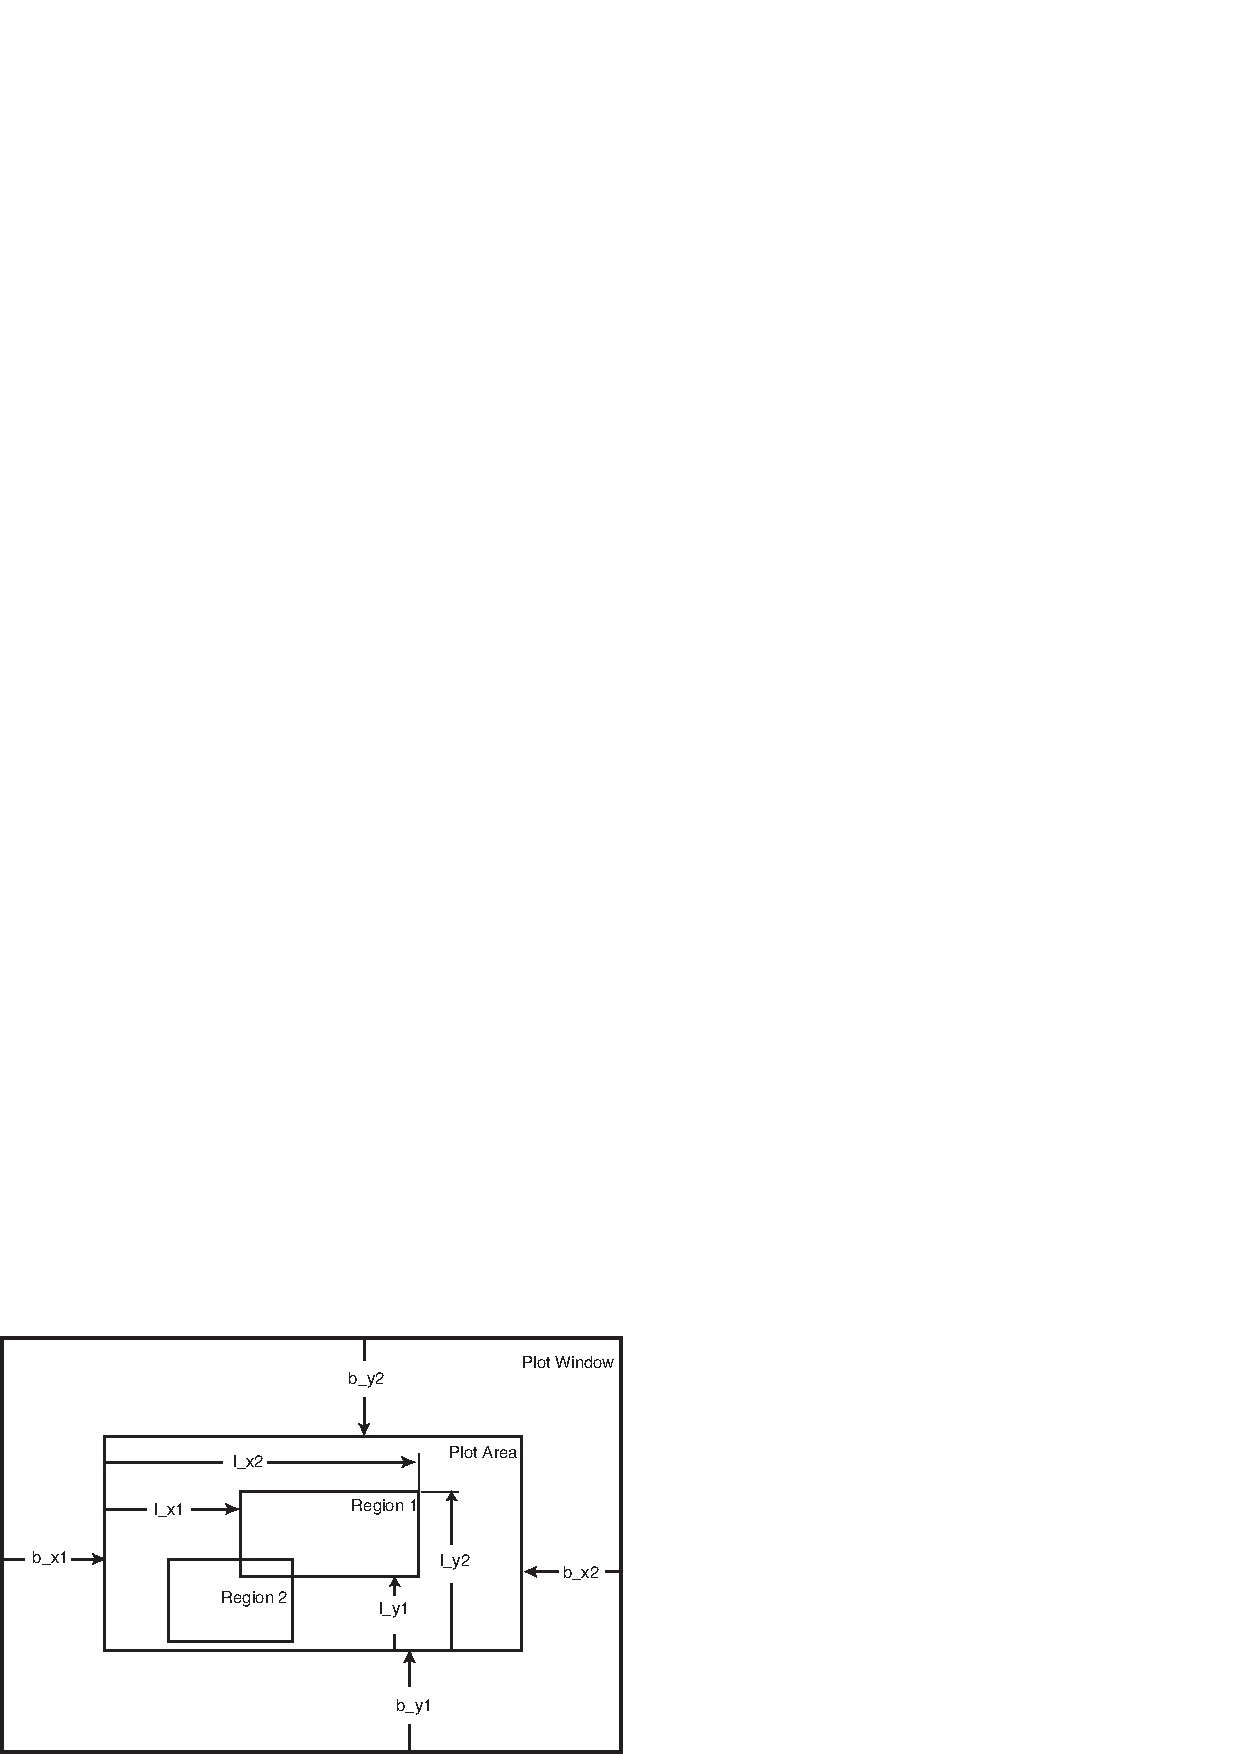
\includegraphics{plot_page.psfig}
  \caption{Regions define where on the plot page plots are placed.}
  \label{f:plot_page}
\end{figure}

Plotting is defined by an initialization file named
\vn{tao_plot.init}.  The first namelist block in the file has a block
name of \vn{tao_plot_page}. This block sets the size of the plot
window (also called the plot page) and defines the ``regions'' where
plots go. The syntax of this block is:
\index{tao_plot_page}    
\index{plot_page!size}
\index{plot_page!border}
\index{plot_page!text_height}
\index{plot_page!title}
\index{region!name}
\index{region!location}
\index{place}
\begin{example}
  &tao_plot_page
    plot_page%size        = <x_size>, <y_size>         ! size in POINTS 
    plot_page%border      = <b_x1>, <b_x2>, <b_y1>, <b_y2>, "<units>"
    plot_page%text_height = <text_height>              !height in POINTS
    plot_page%title(i)    = <string>, {<x>, <y>, "<justify>", "<units>"}
    region(i)%name        = "<region_name>"
    region(i)%location    = <l_x1>, <l_x2>, <l_y1>, <l_y2>  ! % plot area
    place(i)              = "<region>", "<template>"
  /
\end{example}
For example:
\begin{example}
  &tao_plot_page
    plot_page%size        = 700, 800           ! Points
    plot_page%border      = 0, 0, 0, 50, "POINTS"  
    plot_page%text_height = 12.0
    plot_page%title(1)    = "CESR Lattice"
    region(1)%name        = "top"
    region(1)%location    = 0.0, 1.0, 0.5, 1.0
    region(2)%name        = "bottom"
    region(2)%location    = 0.0, 1.0, 0.0, 0.5
    place(1)              = "top", "orbit"
    place(2)              = "bottom", "phase"
  /
\end{example}

\vn{plot_page%size} sets the horizontal and vertical size of the plot
window in \vn{POINTS} units (72 points = 1 inch. Roughly 1 point = 1
pixel). 

\vn{plot_page%border} sets a border around the edges of the
window. As shown in Figure~\ref{f:plot_page} \vn{b_x1}, \vn{b_x2} are
the right and left border widths and \vn{b_y1} and \vn{b_y2} are the
bottom and top border widths respectively.  The rectangle within this
border is called the plot area.

\vn{plot_page%title(i)} set the page title. There are two title areas 
(i = 1,2). If only the title string is given then the other variables 
are set to the defaults \vn{x} = 0.5, \vn{y} = 0.995, \vn{justify} = 
"CC" and \vn{units} = "%PAGE". See the quickplot documentation for 
the \vn{justify} variable syntax.

The plot area is divided up into rectangular regions where plots may
be placed (what defines a plot is discussed below).
\vn{region(i)%name} is the name of a region and my be any character
string. \vn{l_x1}, and \vn{l_x2} define the location of the left and
right edges of the region as a fraction of the plot area width
starting from the left edge of the plot area.  \vn{l_y1} and \vn{l_y2}
define the location of the bottom and top edges of the region as a
fraction of the height of the plot area with respect to the plot
area's bottom edge. Thus, in the above example, region 1 extends from
the left border of the plot area (\vn{region(1)%l_x1} = 0) to the
right border (\vn{region(1)%l_x2} = 0) and vertically from the center
(\vn{region(1)%l_y1} = 0.5) to the top edge (\vn{region(1)%l_x2} =
1.0). Regions may overlap any one can define as many regions as one
likes.

\vn{place(i)} determines the initial placement of plots.

%-----------------------------------------------------------------
\subsection{Templates}\index{Initialization!Plotting!Templates}

As shown in Figure~\ref{f:plot}, a ``plot'' is made up of a collection
of ``graphs'' and a graph consists of axes plus a set of ``curves''.
In the \vn{tao_plot.init} file there needs to be defined a set of
``template plots''. A template plot specifies the layout of a plot:
How the graphs are placed within a plot, what curves are associated
with what graphs, etc. When running \tao, the information in a
template plot may then be transfered to a region using the \vn{place}
command and this will produce a visible plot.

Template plots are defined using namelists with a name of
\vn{tao_template_graph}. The general syntax is:
\index{tao_template_plot}
\index{plot!name}
\index{plot!x}
\index{plot!x_axis_type}
\index{plot!ix_universe}
\index{plot!n_graph}
\index{plot!independent_graphs}
\begin{example}
  &tao_template_plot
    plot%name        = "<plot_name>"
    plot%x           = <qp_axis_struct>
    plot%x_axis_type = "<x_axis_type>"   ! "index" or "s". Default is "index".
    plot%ix_universe = <number> ! used for lat_layout plots
    plot%n_graph     = <n_graphs>
    plot%independent_graphs = <logical>  ! scale graph y-axis independently
  /
\end{example}
For example:
\begin{example}
  &tao_template_plot
    plot%name        = "orbit"
    plot%x%min       =   0
    plot%x%max       = 100
    plot%x%major_div = 10
    plot%x%label     = "Index"
    plot%n_graph     = 2
  /
\end{example}

\vn{plot%x} sets the properties of the horizontal axis. For more
information see the \vn{Quick Plot} documentation on the
\vn{qp_axis_struct}. The major components are
\index{qp_axis_struct!min}
\index{qp_axis_struct!max}
\index{qp_axis_struct!major_div}
\index{qp_axis_struct!minor_div}
\index{qp_axis_struct!label}
\begin{example}
  min        ! Left edge value.
  max        ! Right edge value.
  major_div  ! Number of major divisions. 
             !  Number of major tick marks is one less.
  minor_div  ! Number of minor divisions. 0 = auto choose.
  label      ! Axis label.
\end{example}

\vn{plot%name} is the name that is used with \tao commands to identify
the plot.  

\vn{plot%x_axis_type} sets what is plotted along the
\vn{x-axis}. Possibilities are:
\index{index}
\index{ele_index}
\index{s}
\begin{example}
    "index"      ! Data Index
    "ele_index"  ! Element lattice number index
    "s"          ! Longitudinal position in the lattice.
\end{example}

\vn{n_graph} sets the number of graphs associated with the plot and
each one needs a \vn{tao_template_graph} namelist to define it. These
namelists should be placed directly after their respective
\vn{tao_teamplate_graph} namelists. The general format of the
\vn{tao_template_graph} namelist is:
\begin{example}
  &tao_template_graph
    graph_index           = <number>
    graph%name            = "<graph_name>"
    graph%type            = "<graph_type>"
    graph%box             = <ix>, <iy>, <ix_tot>, <iy_tot>
    graph%title           = "<label>''
    graph%margin          =  <ix1>, <ix2>, <iy1>, <iy2>, "<Units>"
    graph%y               = <qp_axis_struct>
    graph%y2              = <qp_axis_struct>
    graph%n_curve         = <number_of_curves>
    graph%clip            = <logical> ! Clip plot at grpah boundary. default = .true.
    graph%who(i)          = "<who_to_plot>", <sign>
    curve(i)%name         = "<curve_name>"
    curve(i)%data_type    = "<data_type>"
    curve(i)%data_source  = "<source_name>" !source for the data curve points
    curve(i)%units_factor = <factor> ! divide data by this value
    curve(i)%use_y2       = <logical> 
    curve(i)%draw_line    = <logical>
    curve(i)%draw_symbols = <logical>
    curve(i)%ix_universe  = <universe_number> ! default = 0 => use viewed universe
    curve(i)%line         = <qp_line_struct>
    curve(i)%symbol       = <qp_symbol_struct>
    curve(i)%symbol_every = <integer>       ! plot symbol every # datums
    curve(i)%convert      = <Logical>
    curve(i)%ele2_name    = "<element_name>" ! reference element.
  /
\end{example}
For example:
\begin{example}
  &tao_template_graph
    graph_index           = 1
    graph%name            = "x"
    graph%type            = "data"
    graph%box             = 1, 1, 1, 2
    graph%title           = "Horizontal Orbit (mm)"
    graph%margin          =  60, 200, 30, 30, "POINTS"
    graph%y%label         = "X"
    graph%y%max           =  4
    graph%y%min           = -4
    graph%y%major_div     = 4
    graph%n_curve         = 1
    graph%who(1)          = "model", +1
    graph%who(2)          = "design", -1
    curve(1)%data_source  = 'data_array'
    curve(1)%data_type    = "orbit:x"
    curve(1)%units_factor = 1000
    curve(1)%use_y2       = .false.
  /
\end{example}

\vn{graph%name} and \vn{curve%name} define names to be used with
commands. The default names are just the index of the graph or
curve. Thus, in the example above, the name of the curve defaults to
\vn{1} and it would be referred to as \vn{orbit:x:1}.

\vn{graph%who(i)} sets what is plotted by default. For example, if
\vn{graph%who(i) = model - design} then by default the graph will show
the \vn{model} value. Possibilities are:
\index{model}
\index{design}
\index{base}
\index{meas}
\index{ref}
\begin{example}
  "model"     ! model values.
  "design"    ! design values.
  "base"      ! Base values
  "meas"      ! data values.
  "ref"       ! reference data values.
\end{example}
If nothing is specified, the default is to plot \vn{model}. 

\vn{graph%type} is the type of graph. \tao knows about the
following types:
\index{data}
\index{lat_layout}
\index{key_table}
\index{phase_space}
\begin{example}
  "data"         ! Data plots (default) 
  "lat_layout"   ! Schematic showing placement of the lattice elements.
  "key_table"    ! Key binding table for single mode.
  "phase_space"  ! Phase space plots
\end{example}

\vn{graph%box} sets the layout of the box which the \vn{graph} is
placed in. For a definition of what a box is see the Quick Plot
documentation in the \bmad reference manual. In the above example the
graph divides the region into two vertically stacked boxes and places
itself into the bottom one. 

\index{data_array}
\index{var_array}
\index{lat_layout}
The \vn{curve} structure is used to define the number and types of
curves to plot in each graph. \vn{curve%data_source} is the type of
information for the source of the data points. There are the following
types of data sources:
\begin{example}
  "data_array"   ! d1_data is the source of the curve points.
  "var_array"    ! v1_var is the source of the curve points.
  "lat_layout"   ! the lattice is the source.
\end{example}

For a curve with the \vn{curve%data_source} set to \vn{"data_array"} the
possible \vn{curve%data_type} values are the same as the possible
\vn{d1_data%type} values as given in \sref{s:data_types}. If the
\vn{curve%data_source} is \vn{"var_array"} then the possible
\vn{curve%data_type} values are any of the \vn{v1_var} names. This is
what points the curve to the proper data so there needs to be a
corresponding data or var type defined in the initialization file.  If
\vn{graph%type} is \vn{"phase_space"} then \vn{curve%data_source}
determines what planes are plotted. A plane is either:
\index{x}
\index{p_x}
\index{y}
\index{p_y}
\index{z}
\index{p_z}
\begin{example}
  "x"
  "p_x"
  "y"
  "p_y"
  "z"
  "p_z"
\end{example}
For example:
\begin{example}
  curve%data_type = "x-p_x"  ! x-axis - y-axis
\end{example}
The dash \vn{-} is manditory as the spearator between the plane names. 

\vn{curve%convert} is a logical that is only used
with \vn{curve%data_name} = "coupling" and tells \tao to convert the
coupling data into cbar data before plotting.

\vn{curve%draw_symbols} determines whether a symbol is drawn at the
data points. The size, shape and color of the symbols is determined by
\vn{curve%symbol}.

\vn{curve%draw_line} determines whether a curve is drawn through the
data points. The thickness, style (solid, dashed, etc.), and color
is determined by \vn{curve%line}

%-----------------------------------------------------------------
\subsection{Lattice Layout}\index{Initialization!Lattice Layout}

A lattice layout template plot may be defined that draws the lattice
along a straight line with figures for the various elements.
The \vn{tao_template_plot} needed to define a lattice layout looks like:
\index{tao_template_plot}
\index{plot!name}
\index{plot!box_layout}
\index{plot!x!min}
\index{plot!x!max}
\index{plot!n_graph}
\index{tao_template_graph}
\index{graph_index}
\index{graph!name}
\index{graph!type}
\index{graph!title}
\index{graph!box}
\index{graph!ix_universe}
\index{graph!margin}
\index{graph!n_curve}
\begin{example}
  &tao_template_plot
    plot%name        = "<plot_name>"
    plot%box_layout  = <ix>, <iy> 
    plot%x%min       = <number>
    plot%x%max       = <number>
    plot%n_graph     = <number>
  /
  &tao_template_graph
    graph_index       = <number>
    graph%name        = <name>
    graph%type        = "lat_layout"
    graph%title       = "Layout Title"
    graph%box         = <ix>, <iy>
    graph%ix_universe = <integer> ! 0 => use currently viewd universe
    graph%margin      = <ix1>, <ix2>, <iy1>, <iy2>, "<Units>"
    graph%n_curve     = 0
  /
\end{example}
Example:
\begin{example}
  &tao_template_plot
    plot%name       = 'layout'
    plot%x%min      =   0
    plot%x%max      = 100
    plot%n_graph    = 1
  /

  &tao_template_graph
    graph_index       = 1
    graph%name        = 'u1'
    graph%type        = 'lat_layout'
    graph%this_box    = 1, 1
    graph%ix_universe = 1
    graph%margin      = 0.12, 0.12, 0.12, 0.12, '%BOX'
    graph%n_curve     = 0
  /
\end{example}

\index{element_shapes}
\index{shape}
In addition the shapes to be drawn for the various lattice elements need to
be defined using an \vn{element_shapes} namelist whose syntax is:
\begin{example}
  &element_shapes 
    shape(i) = "<key>", "<name>", "<shape>", "<color>", 
                                      "<v_size>", "<print_Label>"
  /
\end{example}
For Example:                 
\begin{example}
  &element_shapes
    shape(1) = "Quadrupole", "Q*",      "Box",  "Red",      30,   T 
    shape(2) = "Quadrupole", "*",       "XBox", "Red",      30,   F 
    shape(3) = "SBend",      "*",       "Box",  "Blue",     15 
    shape(4) = "Wiggler",    "*",       "XBox", "Green",    20 
  /
\end{example}

A figure is drawn for each element in the lattice that matches a
shape. A Match is made if the type of element matches the shape
\vn{<key>} and the name of the element matches the shape
\vn{<name>}. The wildcard ``*'' may be used to denote any number of
characters. Thus, in the example above, \vn{shape(1)} will match to
all quadrupoles whose name begins with ``Q'' and \vn{shape(2)} will
match all quadrupoles. If an element matches more than one shape the
first shape matched will be used. \vn{<shape>} is the shape of the
figure drawn. Valid Shapes are:
\index{BOX}
\index{XBOX}
\begin{example}
  "BOX"           -- Rectangular box
  "XBOX"          -- Rectangular box with an x through it.
\end{example}

\vn{<color>} is the color of the shape. Good colors to use are:
\index{BLACK}
\index{RED}
\index{ORANGE}
\index{MAGENTA}
\index{YELLOW}
\index{GREEN}
\index{CYAN}
\index{BLUE}
\index{PURPLE}
\begin{example}
  "BLACK"
  "RED"
  "ORANGE"
  "MAGENTA"
  "YELLOW"
  "GREEN"
  "CYAN"
  "BLUE"
  "PURPLE"
\end{example}
\vn{<v_size} is the vertical size of the shape in points (72 points =
1 inch). Finally \vn{<print_label>} is a logical indicating whether
the element name is to be printed underneath the figure.



%-----------------------------------------------------------------
\section{Initializing Key Bindings for Single Mode}\index{Initialization!Key Bindings}
\label{s:init_single} 

For single mode the bindings of variables to keys is defined with a
\vn{key_bindings} namelist. There is a maximun of 500 key bingdings.
The syntax is:
\index{key_bindings}
\index{key}
\begin{example}
  &key_bindings
    key(i) = <ele_name> <attrib_name> <delta> <universe> 
          <small_step> <low_lim> <high_lim> <weight> <good_opt> <merit_type>
  /
\end{example}
For example:
\begin{example}
  &key_bindings
  key(1) = "Q1"   "K1"    0.01 "U:0" 1e-5  -10  10  10  T
  key(2) = "DRFT" "L"     0.1  "U:1" 1e-3    0   3   1  F
  key(3) = "Q3"   "TILT"  0.01 "U:2" 1e-5   -1   1   3  T "target"
  /  
\end{example}
For the \vn{i}\Th key \vn{<ele_name>} is the name of a lattice element
in universe \vn{<universe>} and \vn{<attrib_name>} is the attribute to
be varied. If \vn{<unverse>} is ``0'' then the key will vary elements
in all universes. \vn{<delta>} is the change in value when the
appropriate key is depressed. \vn{<small_step>} establishes what a 
``small'' variation of the variable is. 

\vn{merit_type} sets the variable merit is calculated. See
\sref{s:init_var} for more details. the \vn{global%default_key_merit_type} 
sets the default \vn{merit_type}.

If \vn{merit_type} is \vn{"limit"} then \vn{<low_lim>} and
\vn{<high_lim>} establish limits and if the value of the variable goes
outside these limits then the contribution to the merit function is
given by
\index{merit function}
\begin{example}
  merit = <weight> * (var_value - <high_lim>)^2  ! For var_value > <high_lim>
  merit = <weight> * (<low_lim> - var_value)^2   ! Fro <low_lim> > var_value
\end{example}
